\chapter{Szczegółowy opis funkcjonalności i modułów}

W tej części dokumentacji zaprezentowano szczegółowe zrzuty ekranu kluczowych modułów aplikacji, w tym ścieżki autoryzacji, zaawansowanych funkcji klienckich oraz zaplecza administracyjnego. Dla wybranych ekranów zestawiono widoki desktopowe i mobilne, co stanowi dowód na pełne dostosowanie interfejsu do urządzeń mobilnych (RWD).

\section{Ścieżka autoryzacji użytkownika}
Proces logowania i rejestracji został zaprojektowany z myślą o maksymalnej przejrzystości, budowaniu zaufania oraz minimalizacji czasu potrzebnego na założenie konta.

\begin{figure}[H]
    \centering
    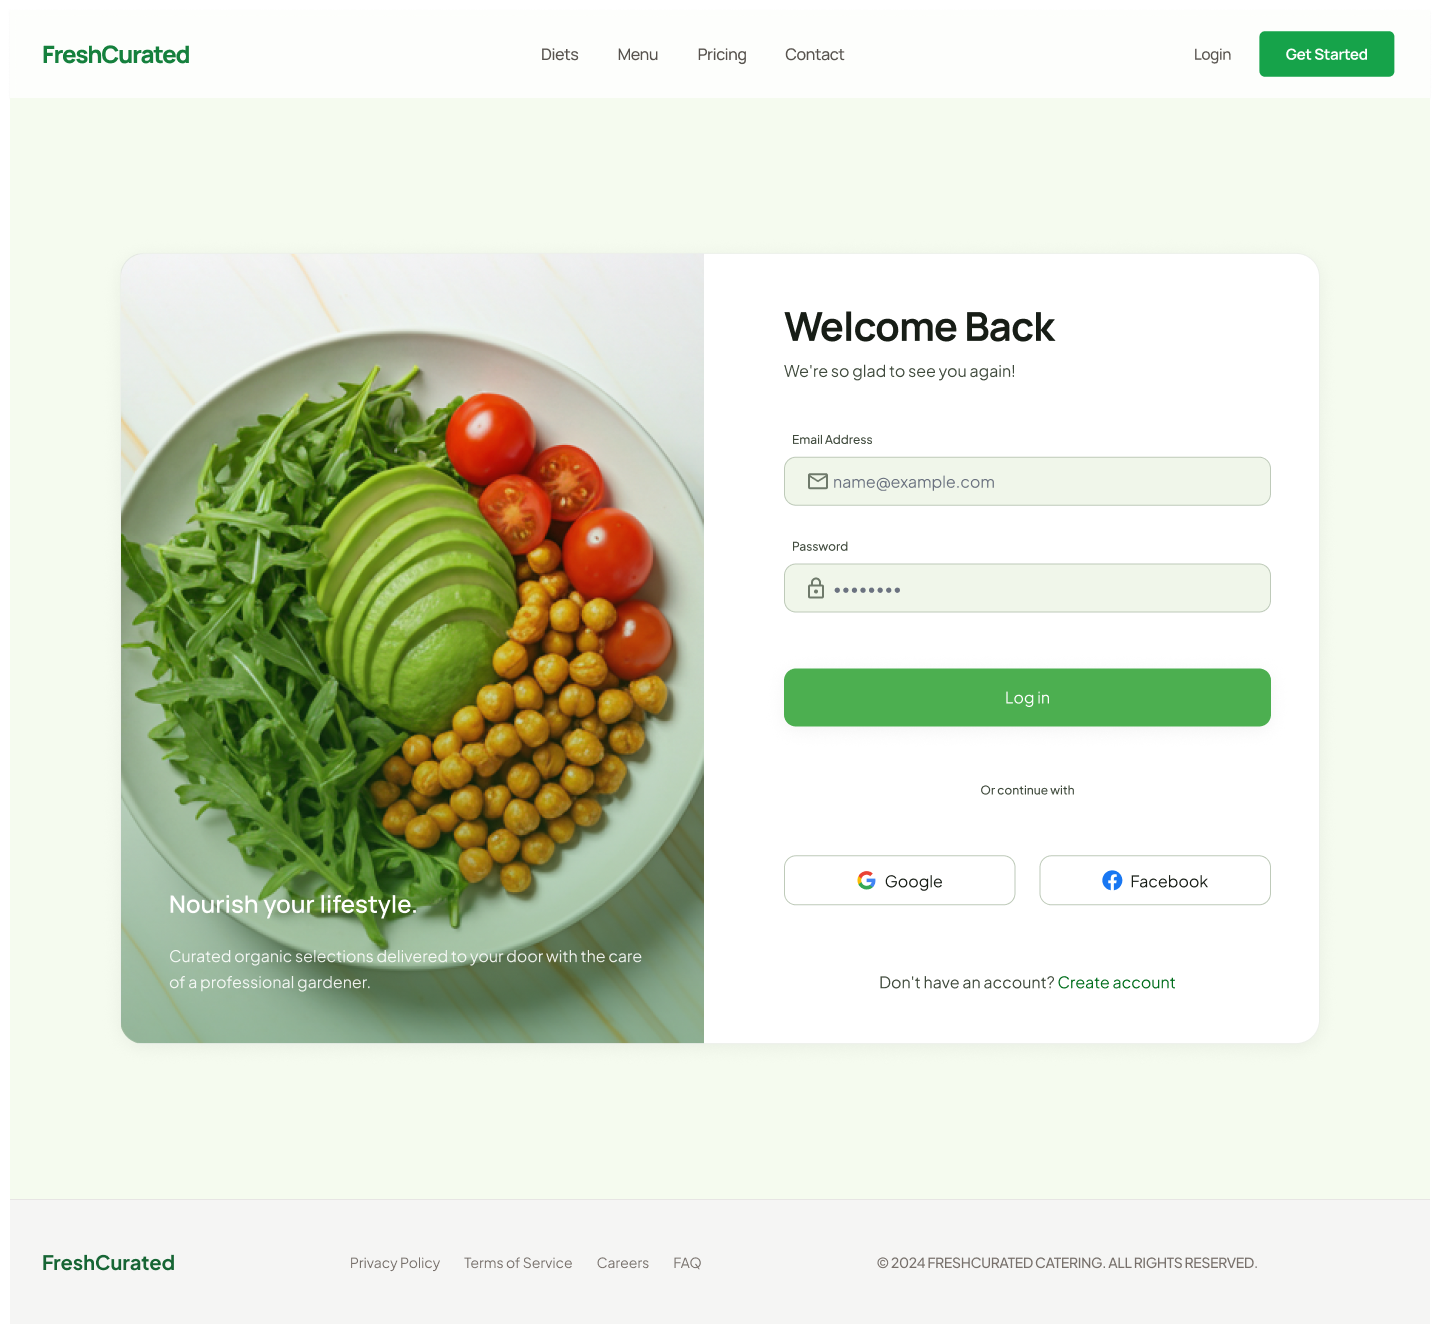
\includegraphics[height=7cm, keepaspectratio]{figures/WelcomeBackLogin.png}
    \hspace{0.5cm}
    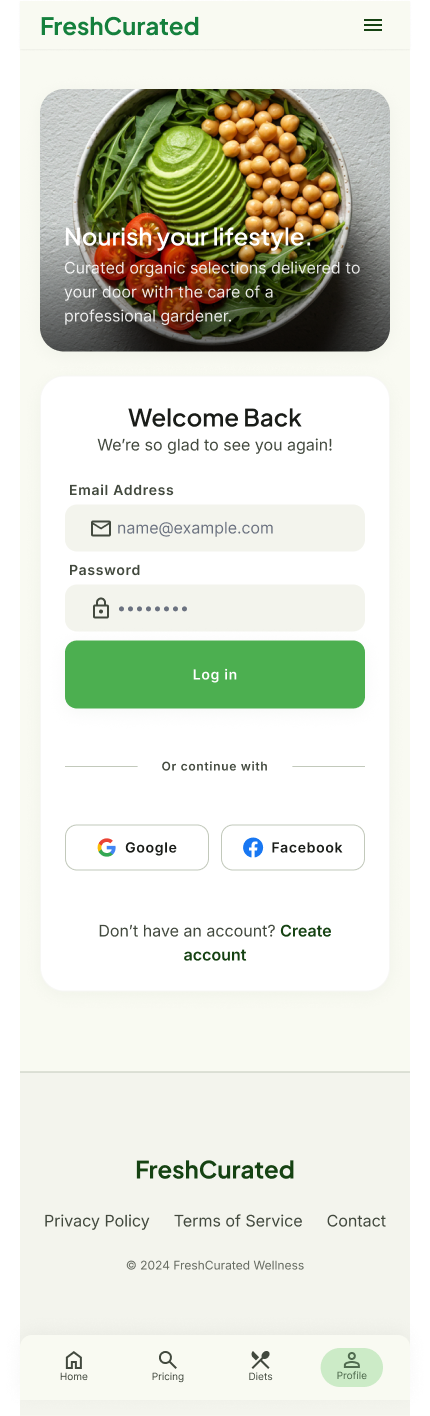
\includegraphics[height=7cm, keepaspectratio]{figures/WelcomeBackLogin-mobile.png}
    \caption{Ekran logowania (desktop i mobile) oferujący standardowe logowanie adresem e-mail oraz szybką integrację z platformami społecznościowymi.}
\end{figure}

Z kolei formularz rejestracji nowego konta posiada wbudowany mechanizm walidacji w czasie rzeczywistym, co znacznie poprawia użyteczność (UX).

\begin{figure}[H]
    \centering
    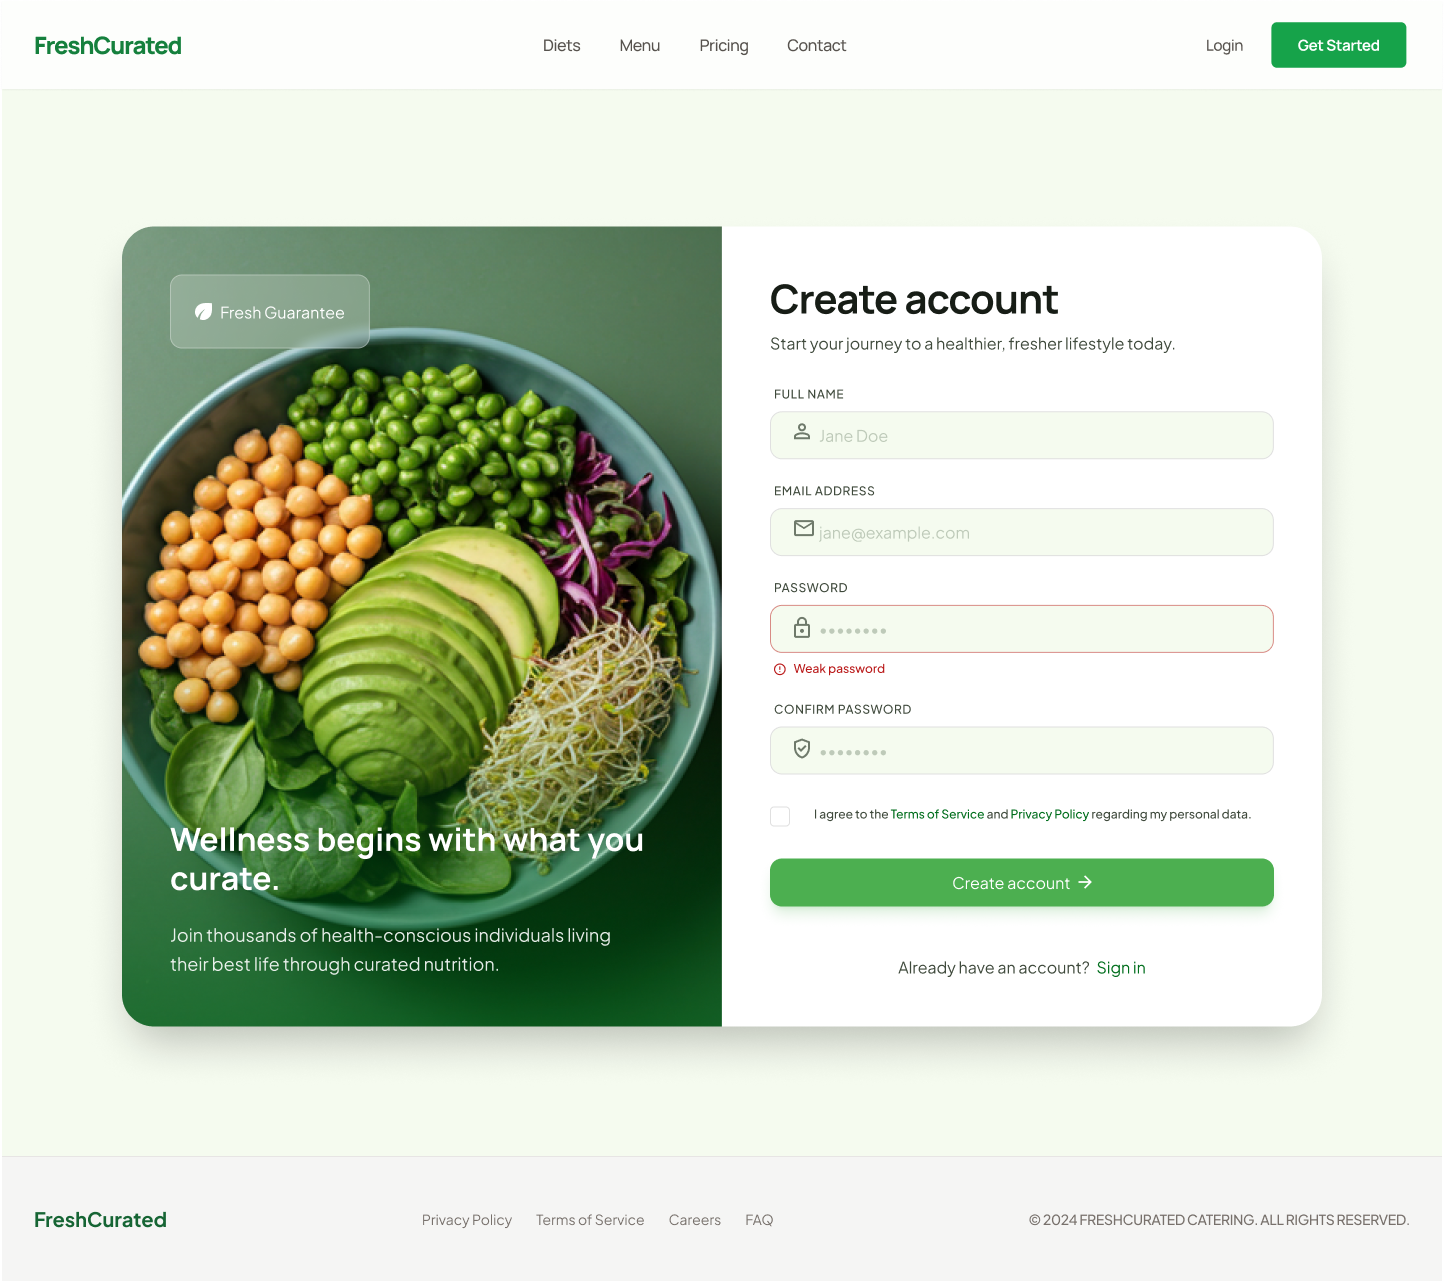
\includegraphics[height=7cm, keepaspectratio]{figures/CreateAccount.png}
    \hspace{0.5cm}
    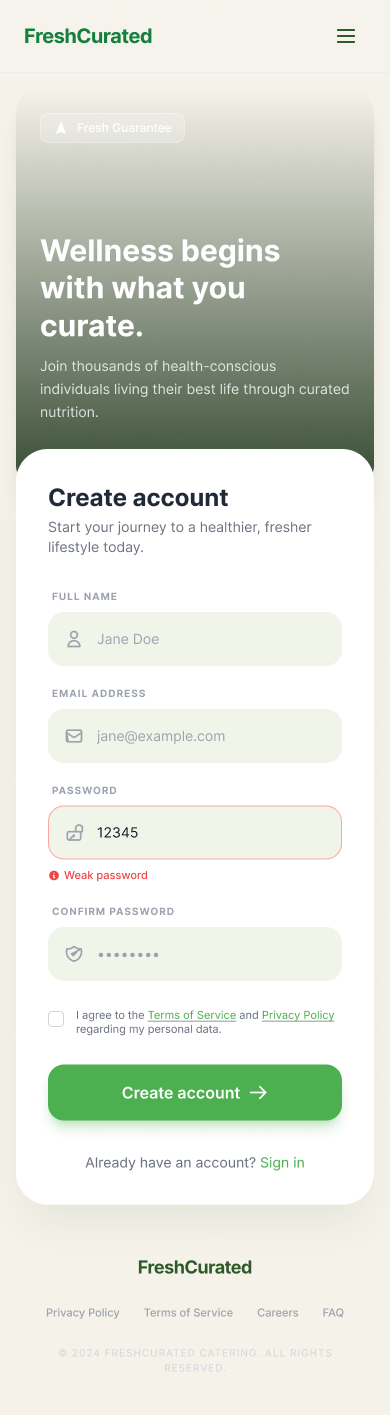
\includegraphics[height=7cm, keepaspectratio]{figures/CreateAccount-mobile.png}
    \caption{Formularz rejestracji z walidacją siły hasła.}
\end{figure}

\section{Rozszerzone funkcjonalności klienckie}
Aplikacja oferuje innowacyjne narzędzia wspierające klienta w świadomym wyborze optymalnego planu żywieniowego.

\begin{figure}[H]
    \centering
    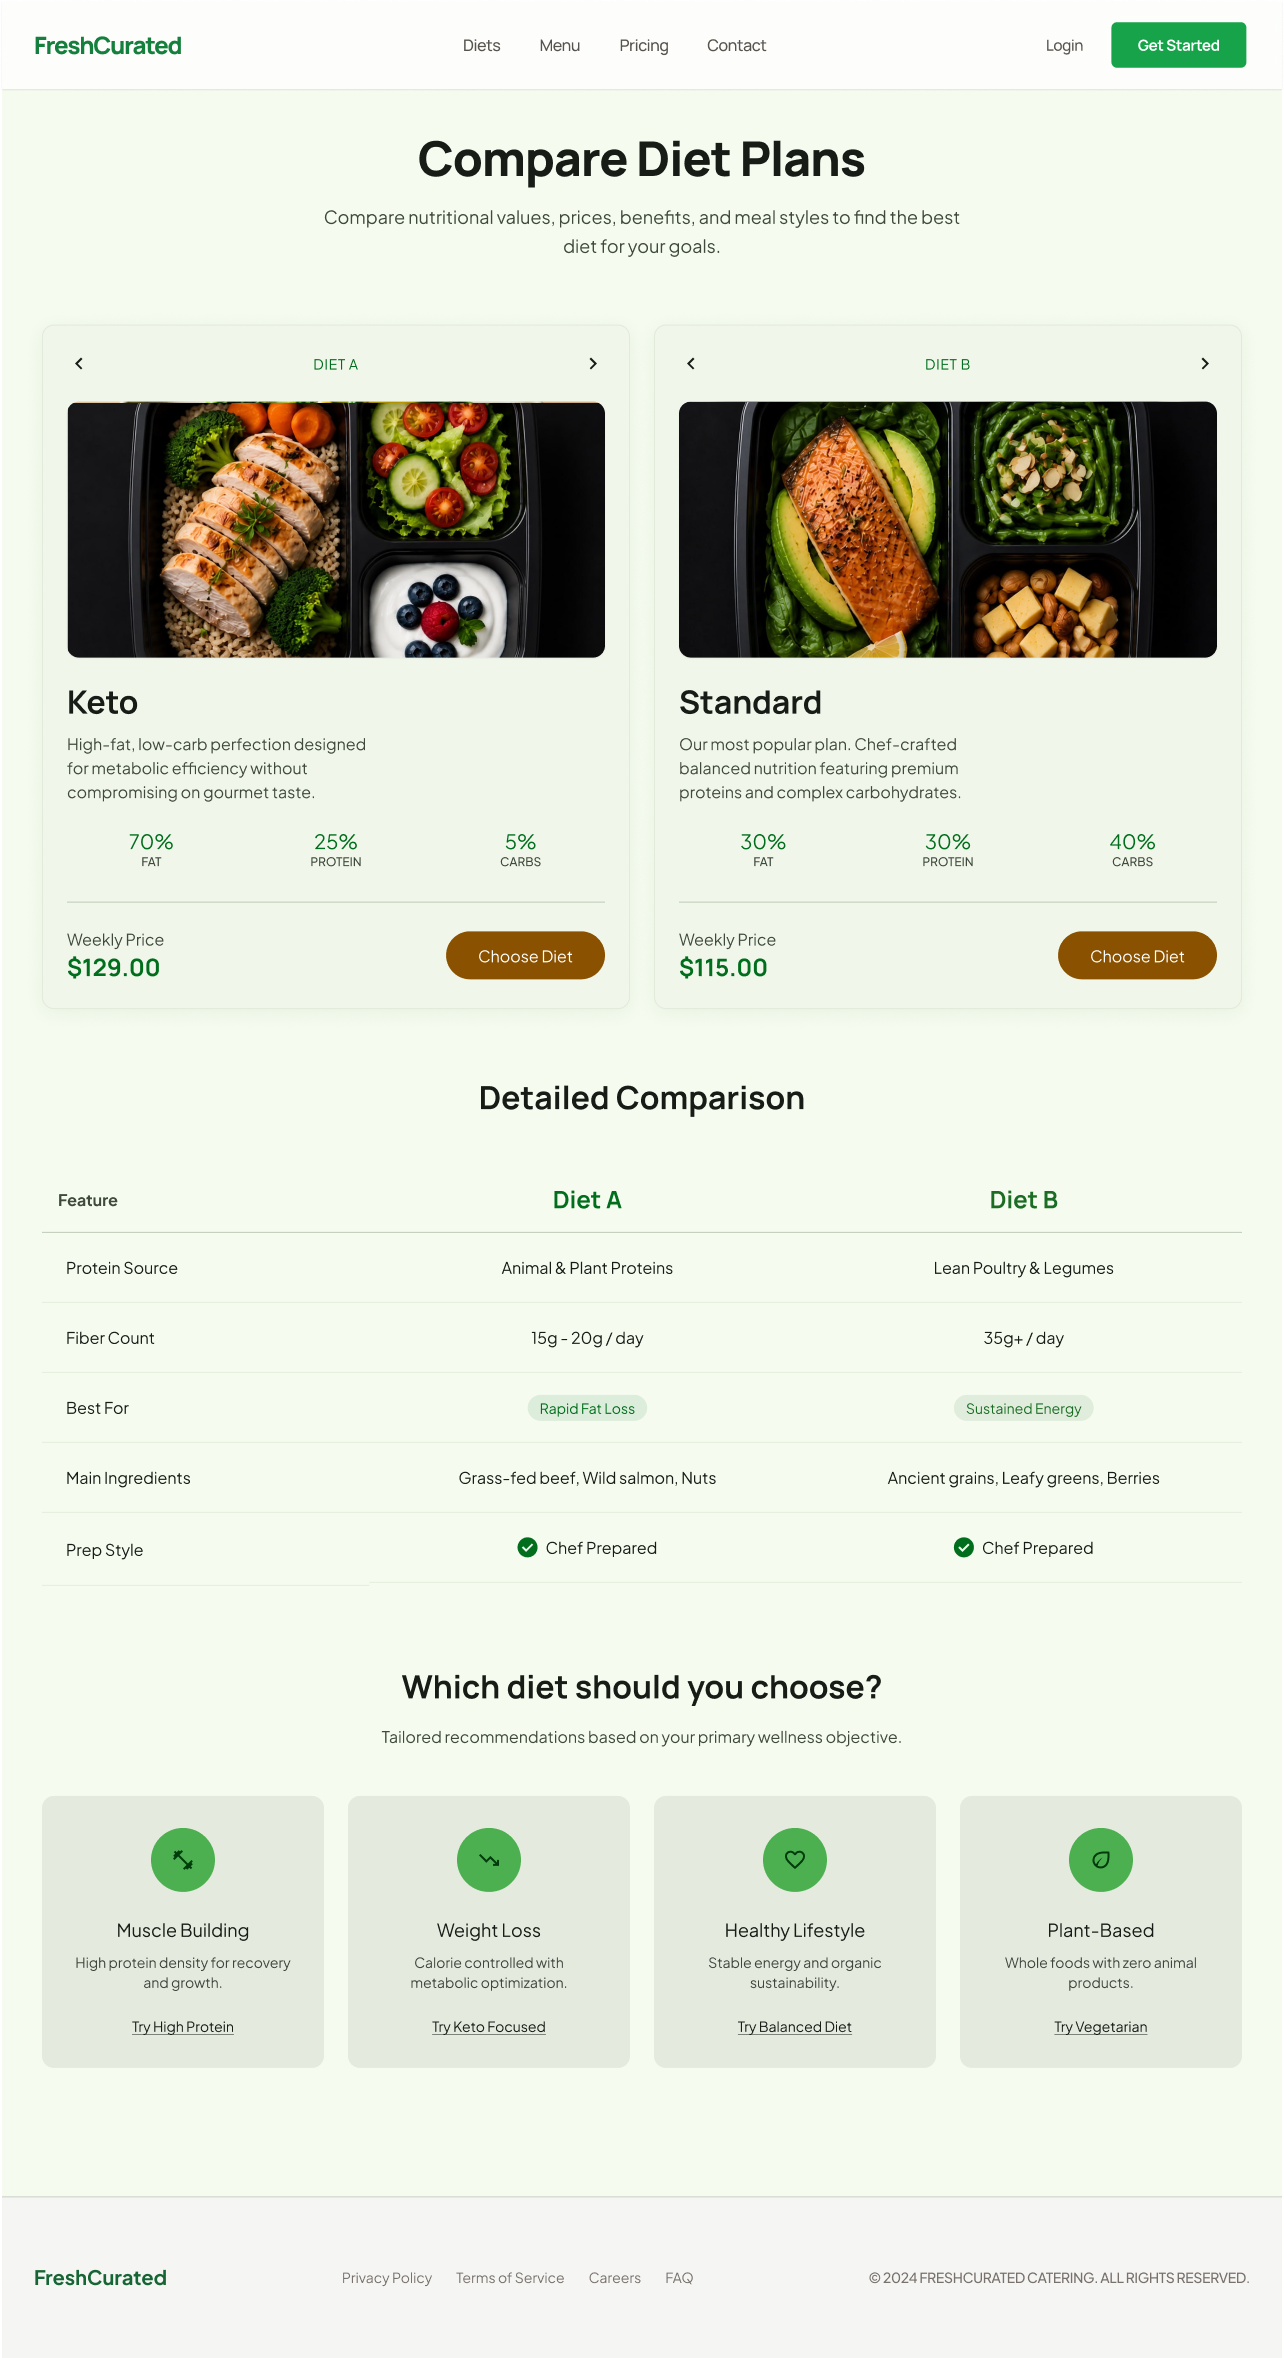
\includegraphics[height=8cm, keepaspectratio]{figures/CompareDiet.png}
    \hspace{0.5cm}
    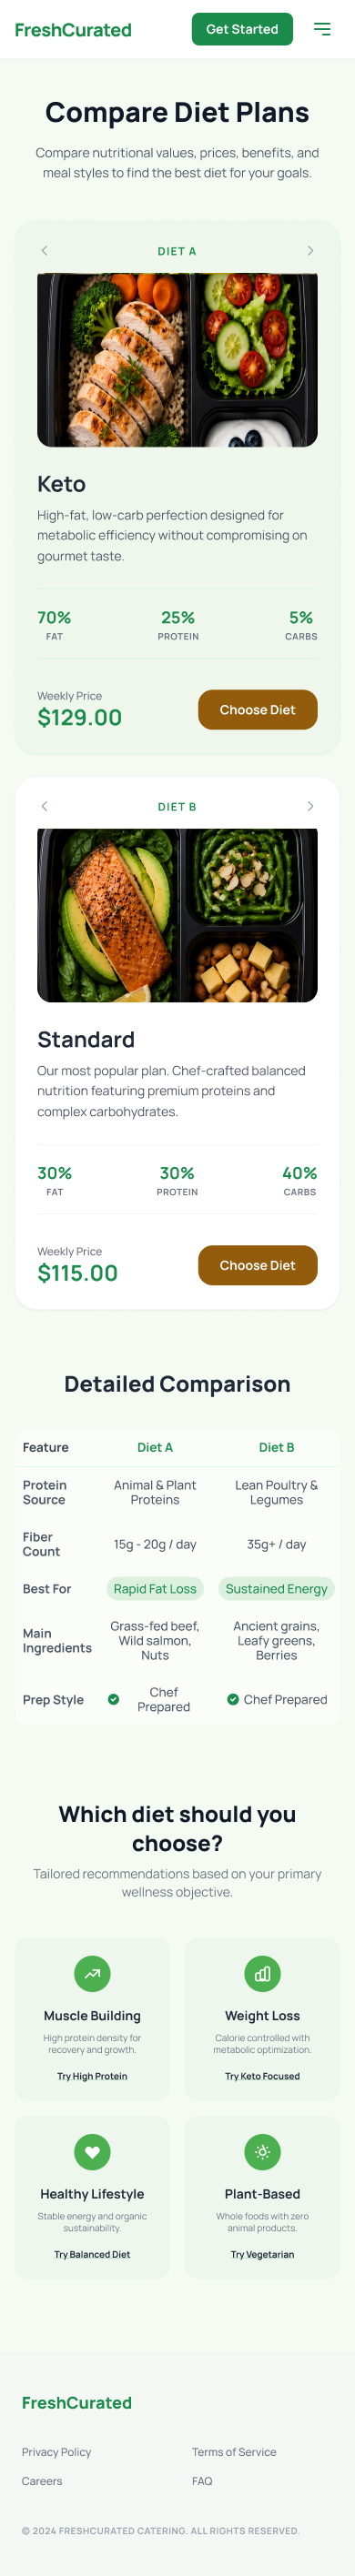
\includegraphics[height=8cm, keepaspectratio]{figures/CompareDiet-mobile.png}
    \caption{Moduł porównywarki diet (desktop i mobile). Pozwala na bezpośrednie zestawienie dwóch planów i ich makroskładników.}
\end{figure}

\section{Moduły administracyjne: Logistyka i Magazyn}
Sprawne działanie firmy cateringowej wymaga zaawansowanych narzędzi dla pracowników zaplecza. Moduły te agregują najważniejsze dane operacyjne.

\begin{figure}[H]
    \centering
    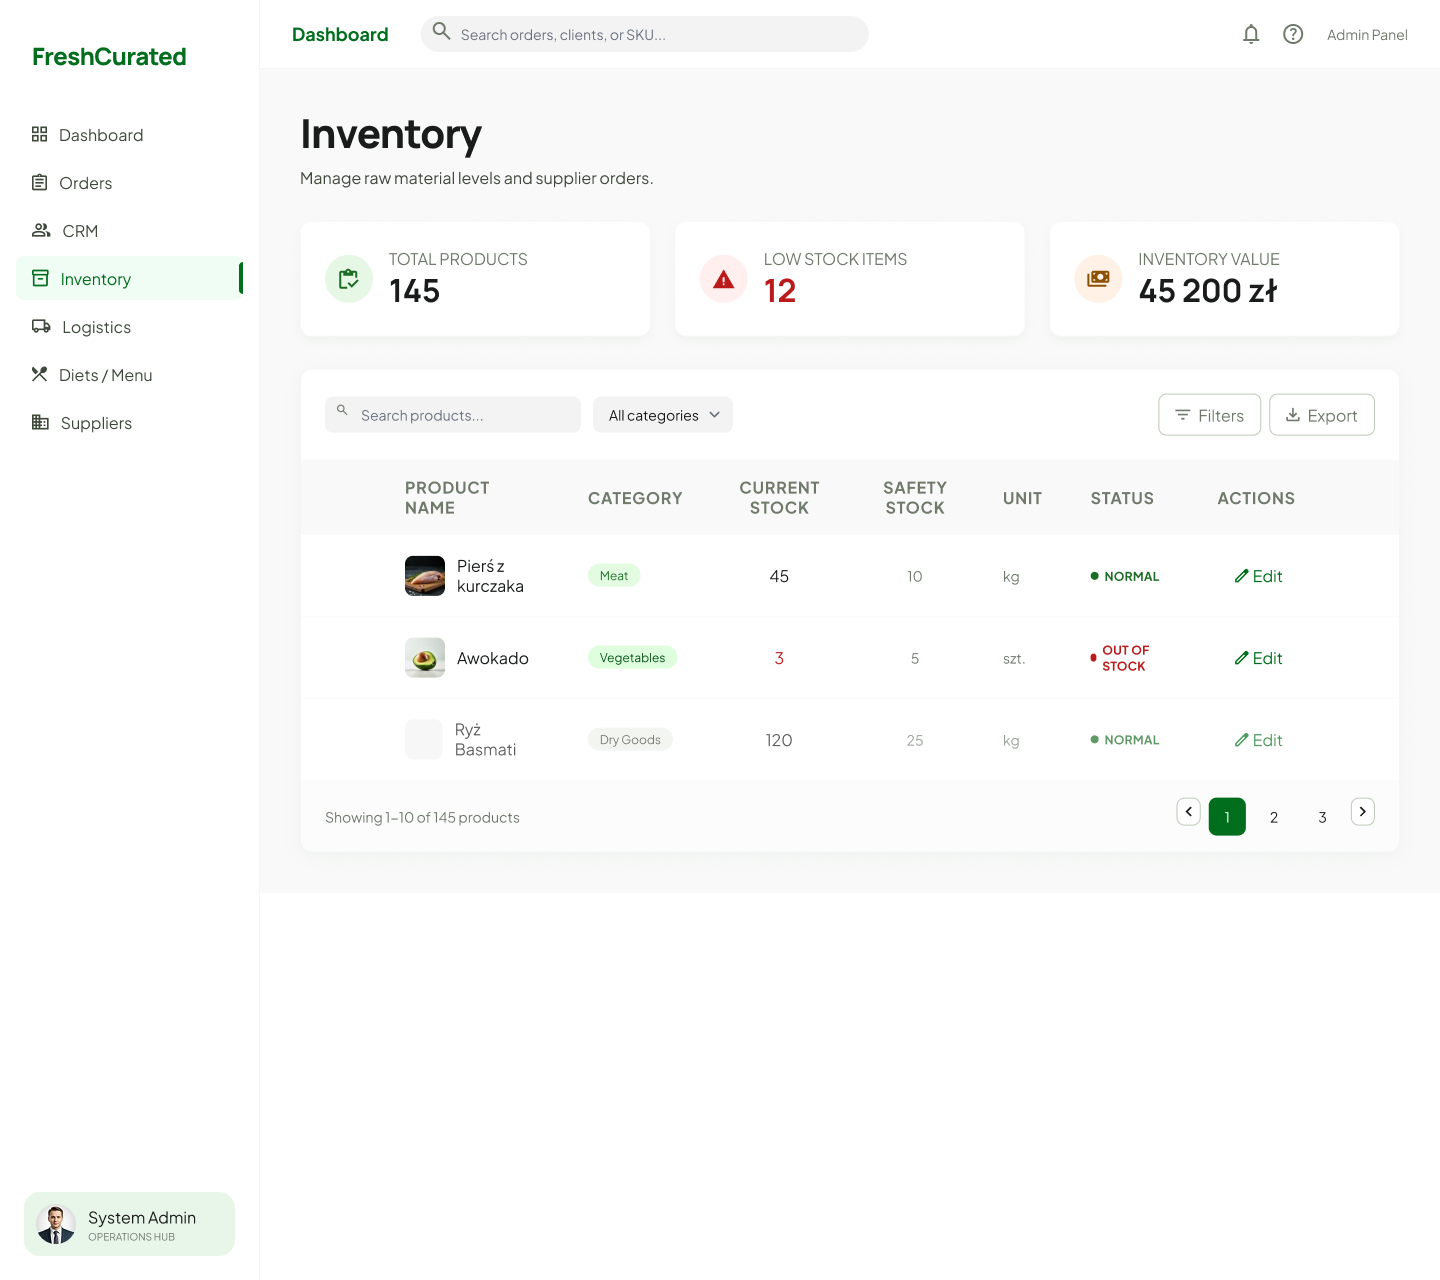
\includegraphics[width=0.85\textwidth, height=8.5cm, keepaspectratio]{figures/admin-inventory.png}
    \caption{Panel zarządzania magazynem (Inventory) z widocznym systemem ostrzegania o niskich stanach magazynowych.}
\end{figure}

Kolejnym kluczowym elementem jest główny panel logistyczny ułatwiający zarządzanie kurierami oraz monitorowanie statusów dostaw na bieżąco.

\begin{figure}[H]
    \centering
    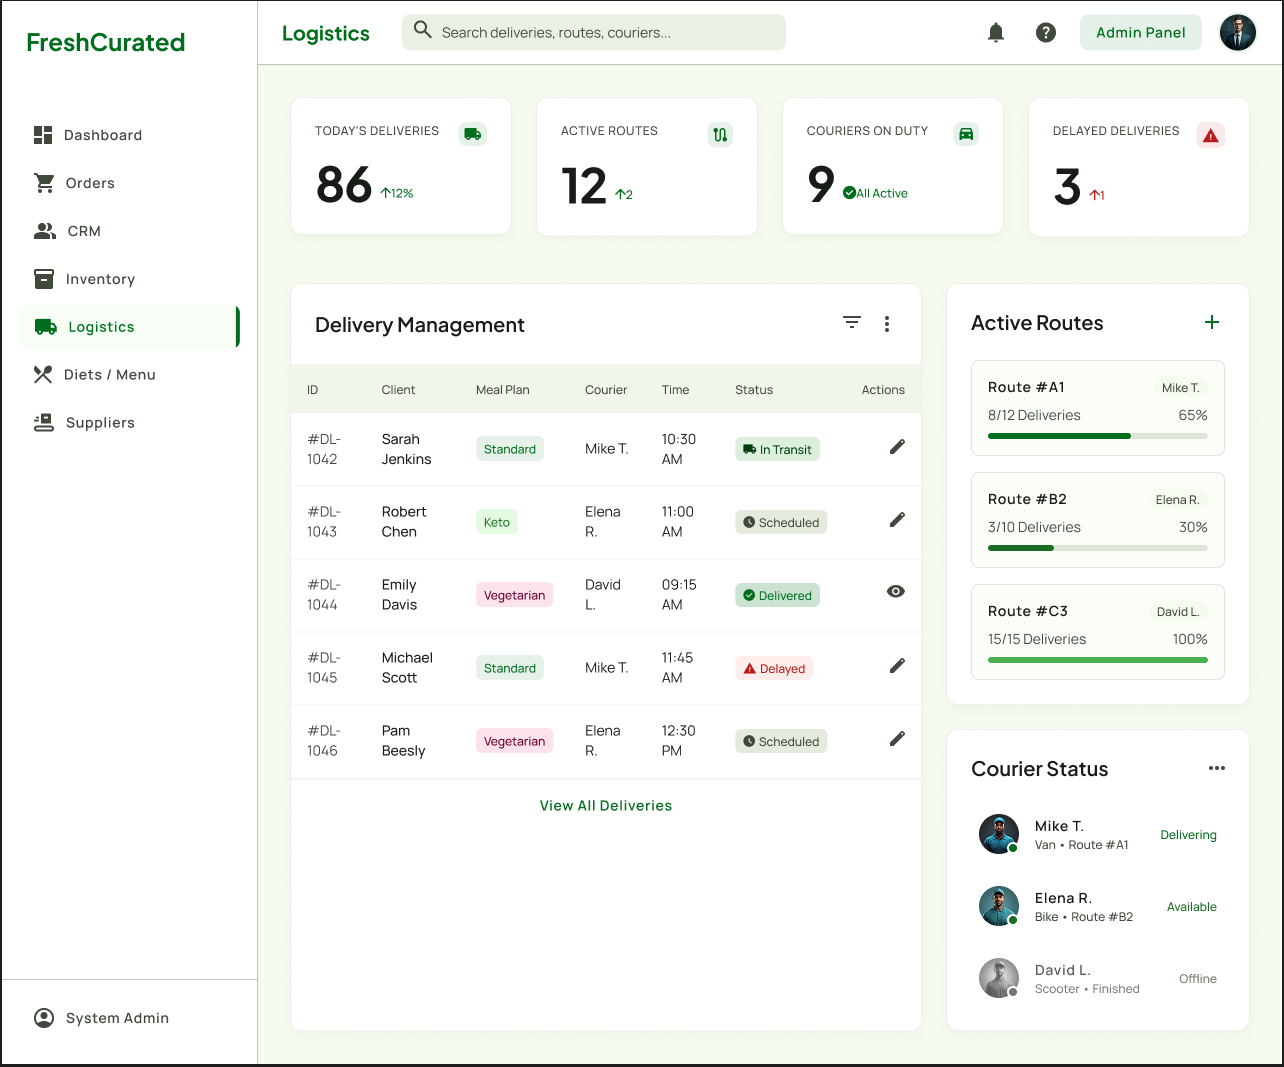
\includegraphics[width=0.85\textwidth, height=8.5cm, keepaspectratio]{figures/admin-logistic.png}
    \caption{Główny panel logistyczny ułatwiający zarządzanie kurierami i trasami.}
\end{figure}

Wsparcie dla logistyki stanowi również interaktywny podgląd na żywo, który ułatwia optymalizację łańcucha dostaw firmy.

\begin{figure}[H]
    \centering
    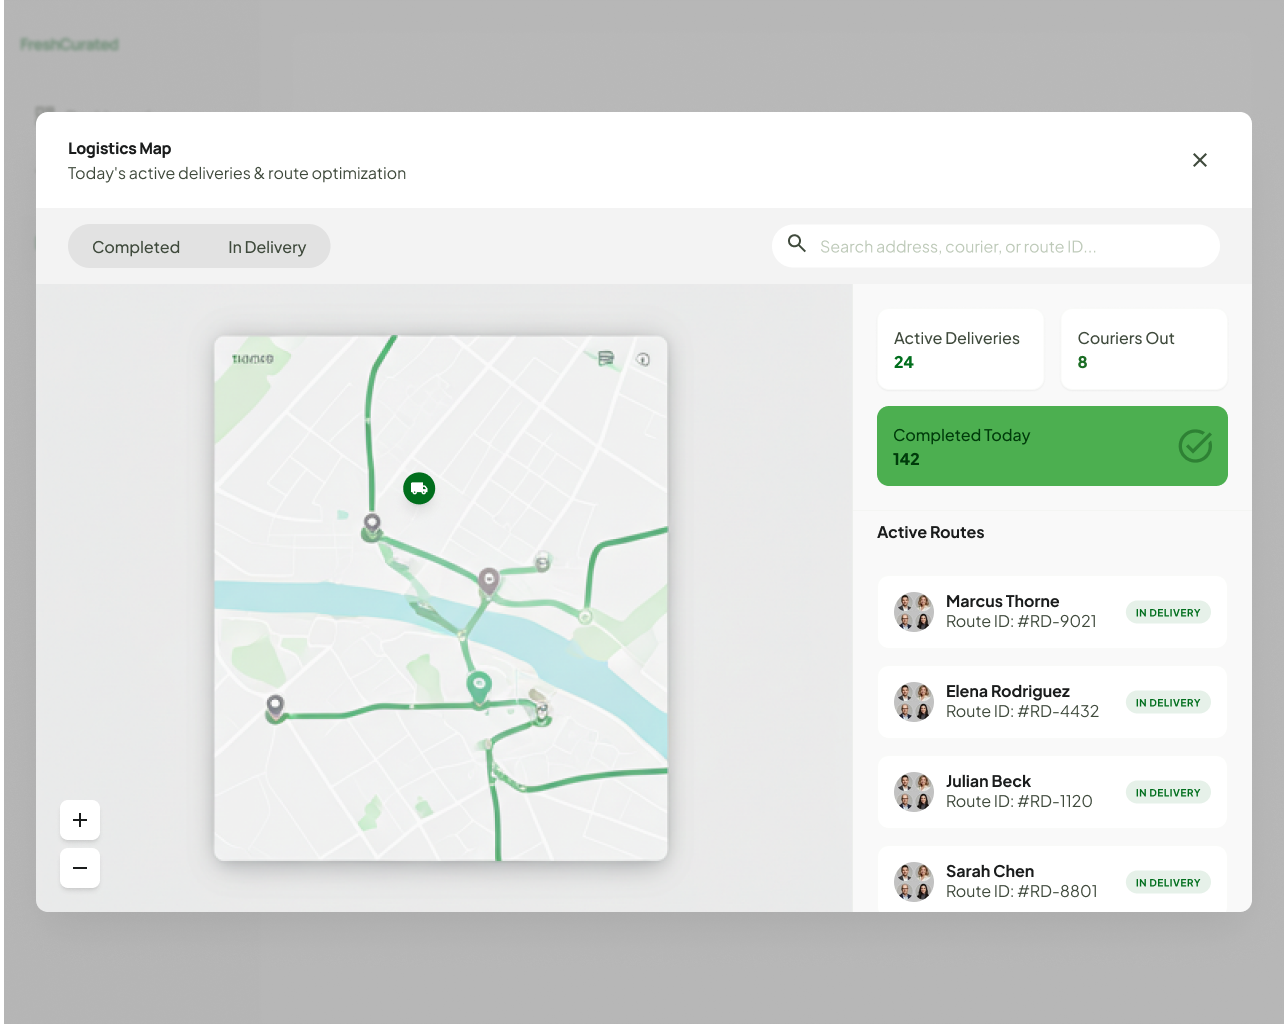
\includegraphics[height=7cm, keepaspectratio]{figures/ModalMap.png}
    \hspace{0.5cm}
    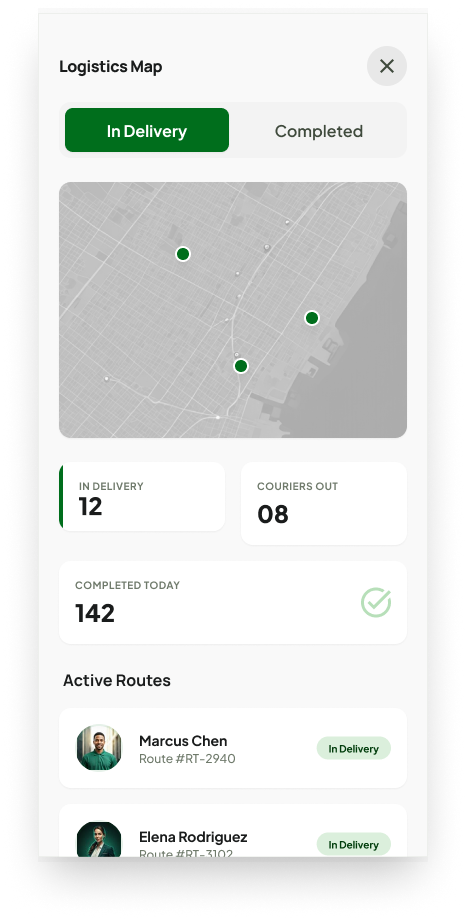
\includegraphics[height=7cm, keepaspectratio]{figures/ModalMap-mobile.png}
    \caption{Interaktywna mapa logistyczna przedstawiająca aktywne trasy kurierów i punkty dostaw.}
\end{figure}